\section{Chronologie}

\subsection{Deux générations de réseau}

La première génération a été entraînée du 7 au 11 mars : un supervisé sur les
seules parties de grands maîtres (4\,749 steps, une époque), puis un second
passage en ajoutant le jeu de données Lichess (9\,755 steps au total), et un
correctif de la tête de policy (15\,752 steps). Elle a ensuite fait 431
itérations de self-play du 10 mars au 4 avril, atteignant 25\,429 steps
d'optimiseur. Ses checkpoints sont conservés dans \chemin{python\_src/checkpoints}.

Le 6 avril, l'architecture change : des blocs Squeeze-and-Excitation sont
insérés dans chaque bloc résiduel et les têtes sont élargies (commit
\code{75977ce}). Une procédure de transfert de poids est écrite
(\chemin{transfer\_weights.py}) et copie 153 des 187 tenseurs de l'ancien
modèle dans la nouvelle architecture. Deux lancements courts du prétraining
Lichess utilisent ces poids transférés, mais leur perte value reste bloquée
autour de 1,9. La lignée retenue est un troisième lancement, reparti de poids
aléatoires, qui produit le checkpoint conservé
\code{2026\_04\_06\_22h25\_SUPERVISED\_LICHESS\_NEW\_MODEL.ckpt}.

\begin{figure}[h]
\centering
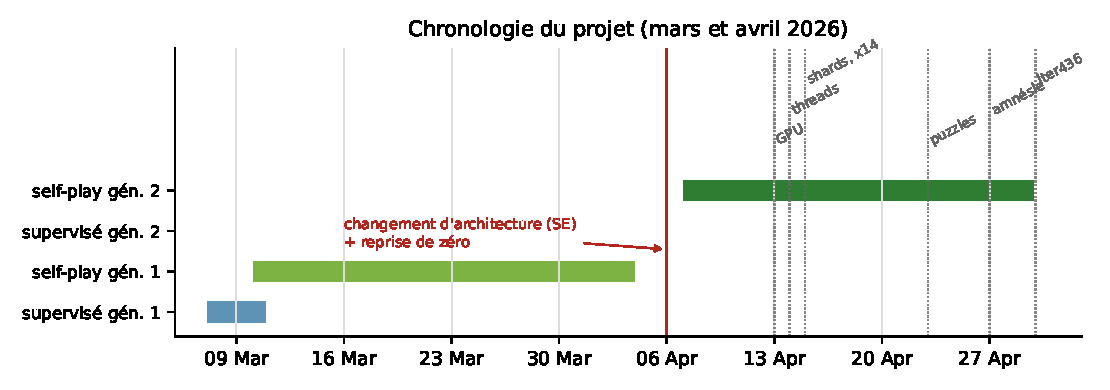
\includegraphics[width=\textwidth]{figures/fig_chronologie.pdf}
\caption{Chronologie du projet en mars et avril 2026. Les événements du
self-play de la génération 2 sont indiqués : self-play batché sur GPU
(13 avril), MCTS multithread (14 avril), buffer en shards et ratio
d'échantillonnage $\times 14$ (15 avril), puzzles tactiques injectés
(23 avril), history dropout (27 avril), dernier checkpoint iter436
(30 avril).}
\label{fig:chronologie}
\end{figure}

\subsection{Les trois phases de la génération retenue}

\begin{table}[h]
\centering
\small
\caption{Phases d'entraînement de la génération retenue. Les positions vues
comptent les époques multiples.}
\label{tab:phases}
\begin{tabularx}{\textwidth}{l >{\raggedright\arraybackslash}p{3.5cm}
    >{\raggedright\arraybackslash}X r r}
\toprule
Phase & Dates (locale) & Données & Positions vues & Steps \\
\midrule
Prétraining Lichess
  & 6 avril, 18 h 49 à 22 h 25
  & 1,2 M de parties, 39,9 M de positions
  & 79,8 M & 19\,495 \\
Affinage grands maîtres
  & 6 avril 22 h 32 à 7 avril 00 h 05
  & 210\,000 parties, 19,5 M de positions
  & 38,9 M & 18\,996 \\
Self-play
  & 7 avril 00 h 34 à 30 avril 09 h 53
  & 211\,000 parties, 5,93 M de positions
  & 105,9 M & 26\,356 \\
\bottomrule
\end{tabularx}
\end{table}

Le prétraining Lichess a en réalité demandé trois lancements successifs
(18 h 49, 19 h 16 et 19 h 33) ; seul le troisième, long de 2 h 52, a produit le
checkpoint conservé. L'affinage sur les grands maîtres a duré 1 h 33. Le
self-play a occupé les 23 jours suivants, en 26 lancements qui reprenaient
chacun le dernier checkpoint du précédent. Le détail de ces 26 lancements est
donné en annexe~A.
